\documentclass{minimal}
\usepackage{epsfig,color}
\usepackage{units}
\usepackage[papersize={576.00bp,432.00bp},text={576.00bp,432.00bp}]{geometry}
\begin{document}
\centering
% Title: glps_renderer figure
% Creator: GL2PS 1.3.8, (C) 1999-2012 C. Geuzaine
% For: Octave
% CreationDate: Wed Oct 29 20:18:47 2014
\setlength{\unitlength}{1pt}
\begin{picture}(0,0)
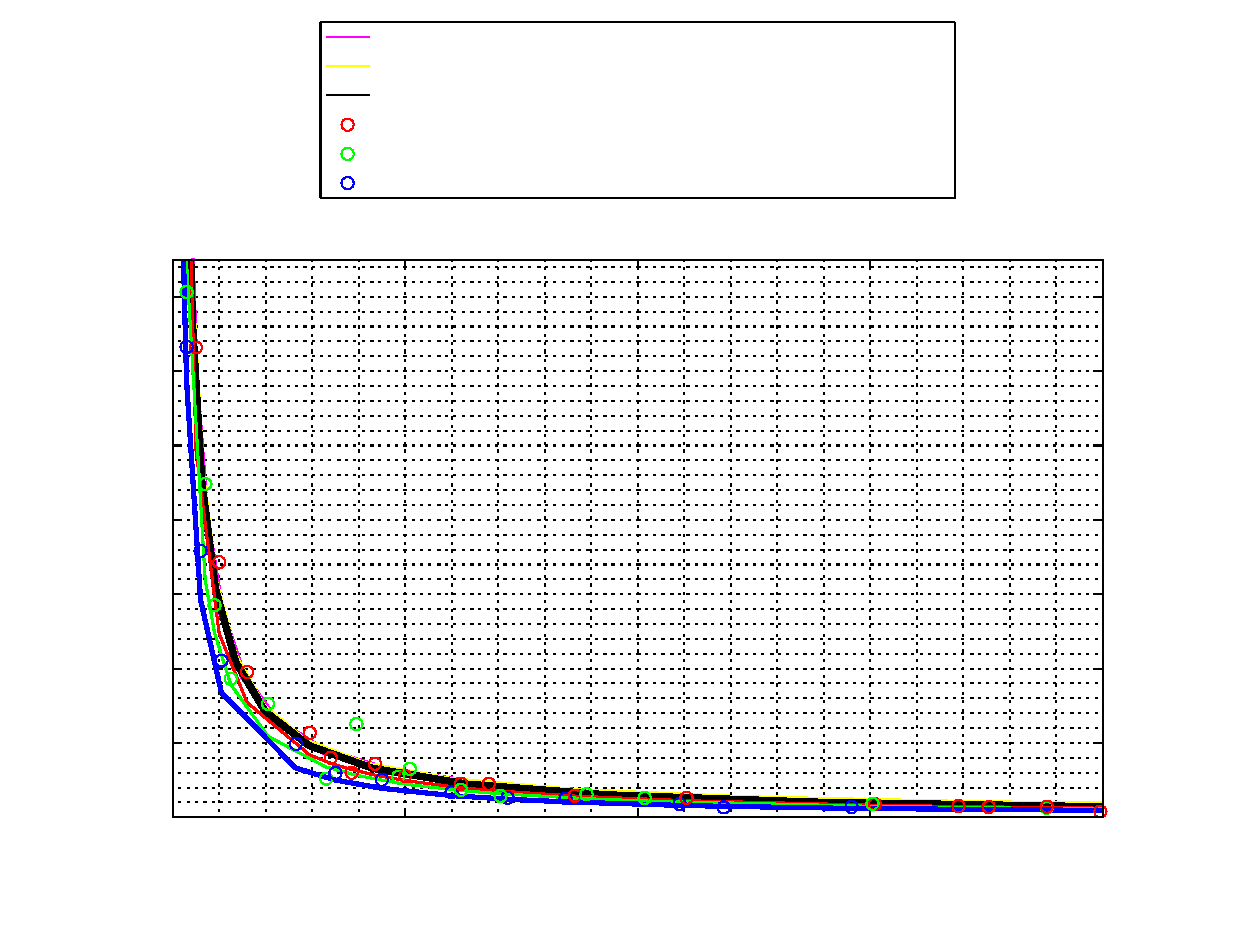
\includegraphics{rpi-inc}
\end{picture}%
\begin{picture}(576,432)(0,0)
\fontsize{10}{0}
\selectfont\put(74.88,42.5252){\makebox(0,0)[t]{\textcolor[rgb]{0,0,0}{{0}}}}
\fontsize{10}{0}
\selectfont\put(186.48,42.5252){\makebox(0,0)[t]{\textcolor[rgb]{0,0,0}{{1}}}}
\fontsize{10}{0}
\selectfont\put(298.08,42.5252){\makebox(0,0)[t]{\textcolor[rgb]{0,0,0}{{2}}}}
\fontsize{10}{0}
\selectfont\put(409.68,42.5252){\makebox(0,0)[t]{\textcolor[rgb]{0,0,0}{{3}}}}
\fontsize{10}{0}
\selectfont\put(521.28,42.5252){\makebox(0,0)[t]{\textcolor[rgb]{0,0,0}{{4}}}}
\fontsize{10}{0}
\selectfont\put(69.8755,47.52){\makebox(0,0)[r]{\textcolor[rgb]{0,0,0}{{0}}}}
\fontsize{10}{0}
\selectfont\put(69.8755,83.2159){\makebox(0,0)[r]{\textcolor[rgb]{0,0,0}{{20000}}}}
\fontsize{10}{0}
\selectfont\put(69.8755,118.912){\makebox(0,0)[r]{\textcolor[rgb]{0,0,0}{{40000}}}}
\fontsize{10}{0}
\selectfont\put(69.8755,154.608){\makebox(0,0)[r]{\textcolor[rgb]{0,0,0}{{60000}}}}
\fontsize{10}{0}
\selectfont\put(69.8755,190.304){\makebox(0,0)[r]{\textcolor[rgb]{0,0,0}{{80000}}}}
\fontsize{10}{0}
\selectfont\put(69.8755,226){\makebox(0,0)[r]{\textcolor[rgb]{0,0,0}{{100000}}}}
\fontsize{10}{0}
\selectfont\put(69.8755,261.696){\makebox(0,0)[r]{\textcolor[rgb]{0,0,0}{{120000}}}}
\fontsize{10}{0}
\selectfont\put(69.8755,297.391){\makebox(0,0)[r]{\textcolor[rgb]{0,0,0}{{140000}}}}
\fontsize{10}{0}
\selectfont\put(298.08,31.5252){\makebox(0,0)[t]{\textcolor[rgb]{0,0,0}{{$I_C [\unit{mA}]$}}}}
\fontsize{10}{0}
\selectfont\put(29.8755,181.38){\rotatebox{90}{\makebox(0,0)[b]{\textcolor[rgb]{0,0,0}{{$r_\pi [\Omega]$}}}}}
\fontsize{10}{0}
\selectfont\put(171.921,422.224){\makebox(0,0)[l]{\textcolor[rgb]{0,0,0}{{\texttt{PHIL\_BJT} $V_{th}= 26,14758\unit{mV}$ $h_{FE} = 365$}}}}
\fontsize{10}{0}
\selectfont\put(171.921,408.164){\makebox(0,0)[l]{\textcolor[rgb]{0,0,0}{{\texttt{SIEMENS} $V_{th}= 25,73160\unit{mV}$ $h_{FE} = 366$}}}}
\fontsize{10}{0}
\selectfont\put(171.921,394.104){\makebox(0,0)[l]{\textcolor[rgb]{0,0,0}{{modelo modificado $V_{th}= 25,78667\unit{mV}$ $h_{FE} = 363$}}}}
\fontsize{10}{0}
\selectfont\put(171.921,380.044){\makebox(0,0)[l]{\textcolor[rgb]{0,0,0}{{transistor 1 $V_{th}= 27,37242\unit{mV}$ $h_{FE} = 361$}}}}
\fontsize{10}{0}
\selectfont\put(171.921,365.984){\makebox(0,0)[l]{\textcolor[rgb]{0,0,0}{{transistor 2 $V_{th}= 27,40305\unit{mV}$ $h_{FE} = 326$}}}}
\fontsize{10}{0}
\selectfont\put(171.921,351.924){\makebox(0,0)[l]{\textcolor[rgb]{0,0,0}{{transistor 3 $V_{th}= 27,74140\unit{mV}$ $h_{FE} = 253$}}}}
\end{picture}
\end{document}
